\documentclass[11pt]{article}
\usepackage{tocloft}
\usepackage{blindtext}
\usepackage{titlesec}
\usepackage[margin=1in]{geometry}
\usepackage{amsmath}
\usepackage{amsthm}
\usepackage{amssymb}
\usepackage{float}
\usepackage{graphics}
\usepackage{graphicx}
\usepackage{helvet}
\usepackage[font=small]{caption}
\usepackage[font=small]{subcaption}
\usepackage[normalem]{ulem}
\usepackage{enumitem}
\usepackage{natbib}
\usepackage{sectsty}
\usepackage{setspace}
\usepackage{hyperref}
\hypersetup{
        colorlinks = true,
        linkcolor = blue,
        filecolor = magenta,            
        urlcolor = cyan,
        pdftitle={Overleaf Example},
        pdfpagemode=FullScreen,
}

\title{Lightweight Clustering Methods on Population SNP Data}
\author{Isaac Thomas}
\setcounter{tocdepth}{5}
\setcounter{secnumdepth}{5}

\newcommand{\code}[1]{\texttt{#1}}

\makeatletter
\renewcommand\paragraph{\@startsection{subparagraph}{5}{\parindent}%
        {3.25ex \@plus1ex \@minus .2ex}%
        {0.75ex plus 0.1ex}% space after heading
        {\normalfont\normalsize\bfseries}}
\makeatother

\makeatletter

\newcommand{\dateformatter}[2]{%
    \textbf{#1} -- \textit{#2}%
}

\newcommand{\dateevent}[2]{%
    \addcontentsline{dates}{section}{#1 -- #2}%
    \dateformatter{#1}{#2}%
}

\newcommand{\listofdates}{%
    \begingroup
    \renewcommand{\contentsname}{List of Dates}
    \let\old@starttoc\@starttoc
    \def\@starttoc##1{%
        \old@starttoc{dates}%
    }
    \tableofcontents%
    \endgroup
}

\makeatother

%\AddToHook{cmd/section/before}{\clearpage}
\renewcommand{\familydefault}{\sfdefault}
\sectionfont{\fontsize{12}{6}\selectfont}
\subsectionfont{\fontsize{10}{6}\selectfont}
\subsubsectionfont{\fontsize{8}{8}\selectfont}
\setstretch{1.5}

\theoremstyle{definition}
\newtheorem{definition}{Definition}
\newtheorem{lemma}{Lemma}
\DeclareSymbolFont{matha}{OML}{txmi}{m}{it}% txfonts
\DeclareMathSymbol{\varv}{\mathord}{matha}{118}
\newcommand{\Setup}{\code{Setup}}
\newcommand{\Prove}{\code{Prove}}
\newcommand{\Verify}{\code{Verify}}
\newcommand{\Sim}{\code{Sim}}
\setlistdepth{100}
\newenvironment{myenum}%
{\pointedenum\begin{enumerate}}%
{\end{enumerate}}
\begin{document}
\maketitle

% \section{TODO}
% \begin{itemize}
%     \item download \code{plink} (right version) and get it to run $\checkmark$
%     \item download pruned vcf data for chromosome 19 $\checkmark$
%     \item get PCA results $\checkmark$
%         \begin{itemize}
%             \item map each row of PCA data to its population code and subpopulation code $\checkmark$
%         \end{itemize}
%     \item build and run $k$-means
%     \begin{itemize}
%         \item plot silhouette score vs $k$ $\checkmark$
%         \item compute silhouette score of optimal clustering $\checkmark$
%         \item plot the optimal clustering $\checkmark$
%         \begin{itemize}
%             \item label/color points by their population/subpopulation $\checkmark$
%             \item map each point to plot to its shape (true label) and color (true label) $\checkmark$
%             \item label/color points by their population/subpopulation $\checkmark$
%         \end{itemize}
%     \end{itemize}
%     \item build and run hierarchical clustering
%     \begin{itemize}
%         \item 
%         \item plot optimal clustering using ward linkage $\checkmark$
%         \item label/color points by their population/subpopulation $\checkmark$
%         \item plot dendrogram $\checkmark$
%         \item get dendrogram sorted out $\checkmark$
%     \end{itemize}
% \end{itemize}
\section{Introduction}\label{sec:intro}
\subsection{Motivation}
\noindent Single Nucleotide Polymorphisms (SNPs) have had massive intergenerational effects on human phenotypes. Such impact renders SNP data useful in describing phenotypes to an extent that allows informative clustering. As biologically/probabilistically informed methods for this task can be more space/computation intensive, we attempt to determine the simplest clustering method that can informatively cluster SNP data with the goal of capturing population demographics. Using the 1000 genomes dataset, we compare $k$-means and hierarchical clustering regarding how much structure they can discern without substantial biological or probabilistic information/assumptions. We also highlight limitations of this work and avenues for future research.

\section{Materials, Methods, and \href {https://github.com/0xArsi/snp-clustering.git}{Code Availability}}\label{sec:methods}
\subsection{Data \& Preprocessing}\label{subsec:data}
We used the 1000 Genomes Dataset \cite{1000genomes}, which consists of SNPs from thousands of individuals categorized by population. To save time, we used only SNPs from chromosome 19. We used data that was already LD-pruned to eliminate SNPs strongly correlated for reasons unrelated to population traits. We then performed principal component analysis with \code{plink},  keeping 4 principal components. Given our SNP data matrix $X$, PCA computes the singular value decomposition $X = \textbf{U} \boldmath{\Sigma} \textbf{V}^\top $, where the rows of the lower-dimensional $\textbf{U}$ are the transformed data in the basis determined by the columns of $\textbf{V}^\top$. The columns of $\textbf{V}^\top$ contain the contribution of each SNP to the data.
\subsection{Clustering Methods Used}
\noindent We first used $k$-means clustering with Lloyd's algorithm \cite{lloyd} for iterative centroid computation and point-cluster reassignment. For this experiment and the following one, we used silhouette score \cite{silhouette} as a measurement of cluster quality, which measures the "tightness" of the inferred clusters. We tuned $k$ to maximize silhouette score (500 iterations per clustering) using \code{scikit-learn} \cite{sklearn}.

\noindent For hierarchical clustering, we used an \textit{agglomerative} approach which treats each point as a cluster and repeatedly merges the two "closest" clusters until some stopping criterion is met. We determined the closest clusters at each iteration via the following methods for two clusters $A$ and $B$:
\begin{itemize}
    \item single linkage \cite{singlecomplete}: take the minimum distance between any point in $A$ and any point in $B$.
    \item complete linkage \cite{singlecomplete}: take the maximum distance between any point in $A$ and any point in $B$.
    \item average linkage \cite{average}: take the average distance between any point in $A$ and any point in $B$.
    \item Ward linkage \cite{ward}: take the resulting change in intra-cluster variance by merging $A$ and $B$.
\end{itemize}

\noindent Using \code{scikit-learn}, we tuned all hierarchical approaches by distance threshold, which is the distance between two clusters that renders them too far away to merge (stopping criterion).

\section{Discussion}\label{sec:discussion}
\subsection{Results}\label{subsec:comparison}
\noindent We found that $k$-means clustering and hierarchical clustering performed similarly in extracting insight from the PCA-transformed SNP data. Through hyperparameter tuning w.r.t. silhouette score, $k$-means discerned an optimal 5 clusters, which was near the correct number of populations in the data (6). Figure $\ref{fig:kmeanspop}$ shows the resulting visualization, with clear separation between most of the big populations. 

\begin{figure}
    \begin{center}
        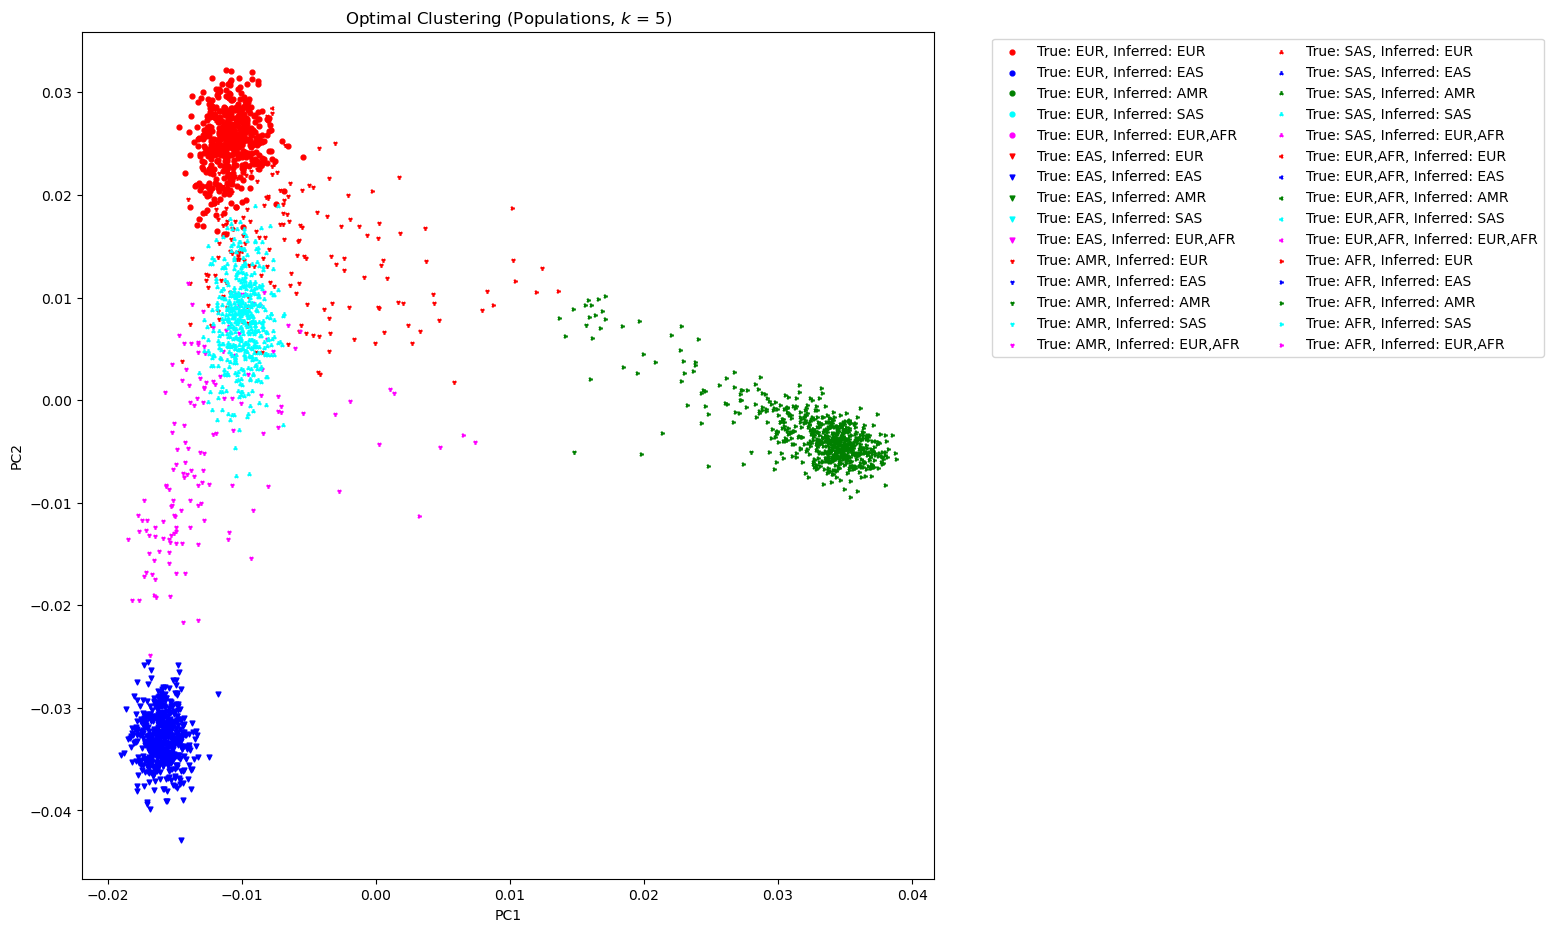
\includegraphics[scale=0.35]{img/snp_clustering_report_34_1.png}
    \end{center}
    \caption{Results of tuning $k$ in the clustering to something consistent with the number of subpopulations. The shape of each point is its true subpopulation, and its color is the subpopulation it was assigned to.}
    \label{fig:kmeanspop}
\end{figure}

\noindent $k$-means attained a silhouette score of $\sim 0.75$ using the optimal value of $k$. A score near 0 would indicate lots of overlapping clusters, and a score below 0 would indicate a very large number of misassignments. As silhouette score lies in $[-1, 1]$, this indicates that the clustering is decently tight. Although there is decent separation between the populations, there is little separation within them. This may foreshadow difficulty in discerning subpopulation structure, which turned out to be the case as shown in figure 2.

\begin{figure}
    \begin{center}
        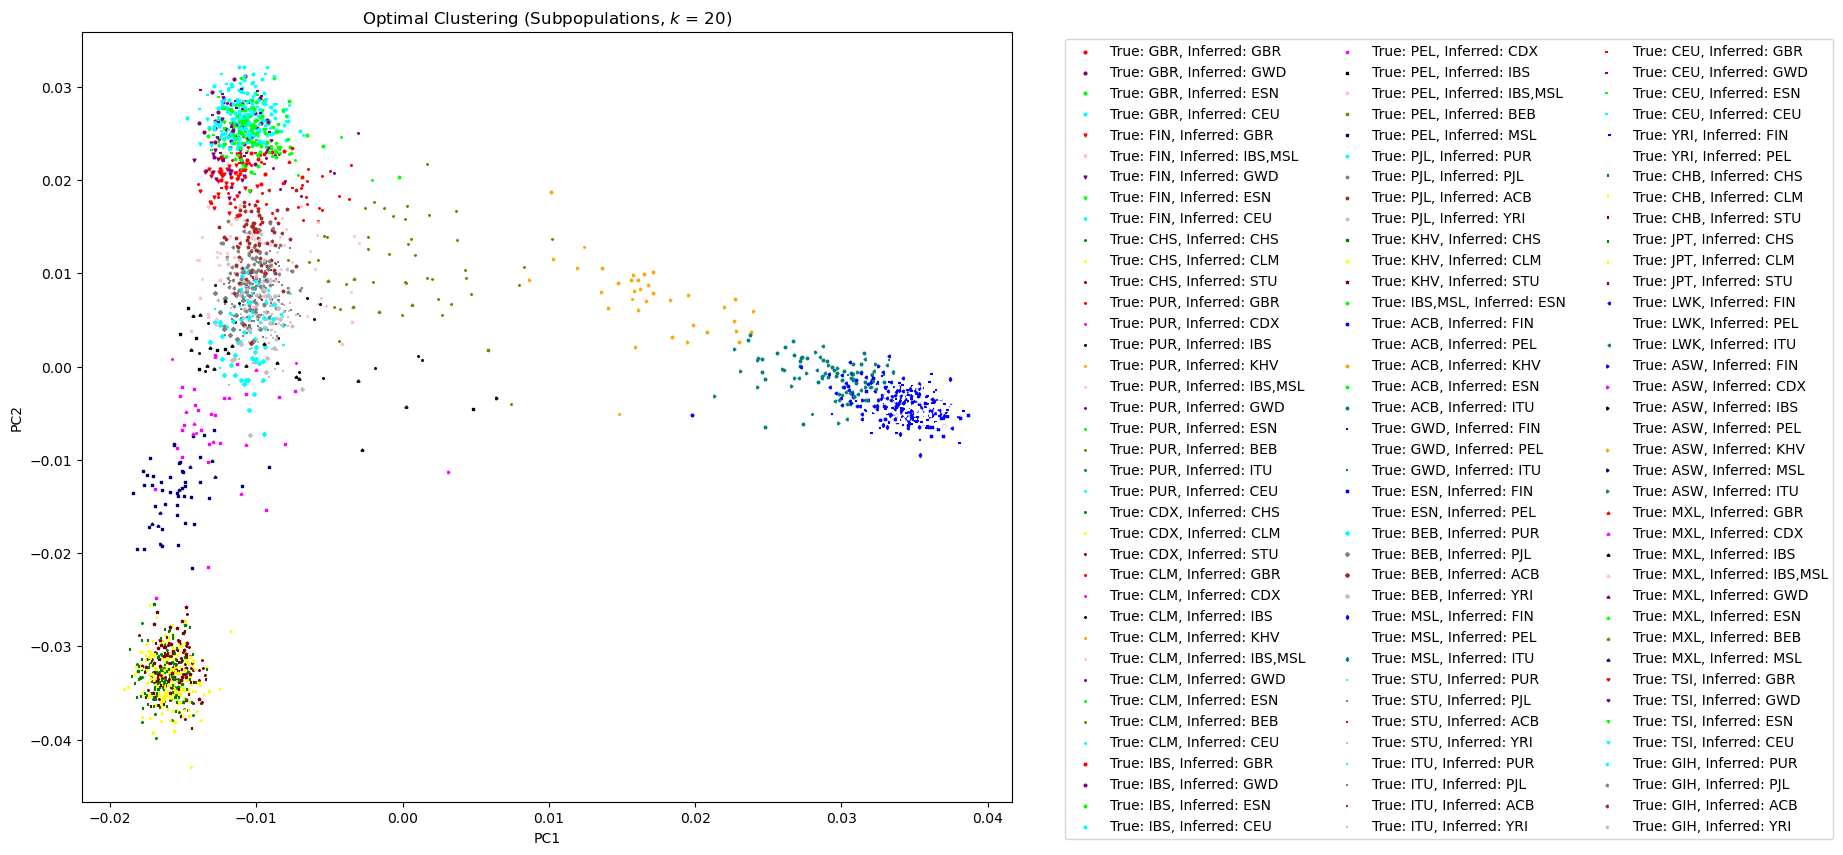
\includegraphics[trim={0 0 0 7cm},scale=0.35]{img/snp_clustering_report_38_1.png}
    \end{center}
    \caption{Results of $k$-means clustering on the the LD-pruned SNP 1000 Genomes data (Chr 19). The shape of each point is its true subpopulation, and the color indicates the subpopulation inferred by $k$-means.}
    \label{fig:kmeanssubpop}
\end{figure}

\noindent We deliberately tuned the clustering to select the optimal $k$ in between 20 and 30 (true number of subpopulations was 27), and we ended up with a very low silhouette score and many subpopulation-level misassignments of points in the same population (Figure $\ref{fig:kmeanssubpop}$). The resulting silhouette score for optimal $k=20$ was $\sim 0.34$, which agrees with the notion of many subpopulation clusters overlapping.

\noindent The best hierarchical methods (Ward linkage, average linkage) attained silhouette scores in the same range as $k$-means, settling on a tuned distance threshold yielding 5 clusters. The truncated dendrogram of the Ward clustering depicts this in figure $\ref{fig:hierpop}$. Having settled on such a low $k$, tuning method did not result in extra insight about subpopulation structure.

\begin{figure}
    \begin{center}
        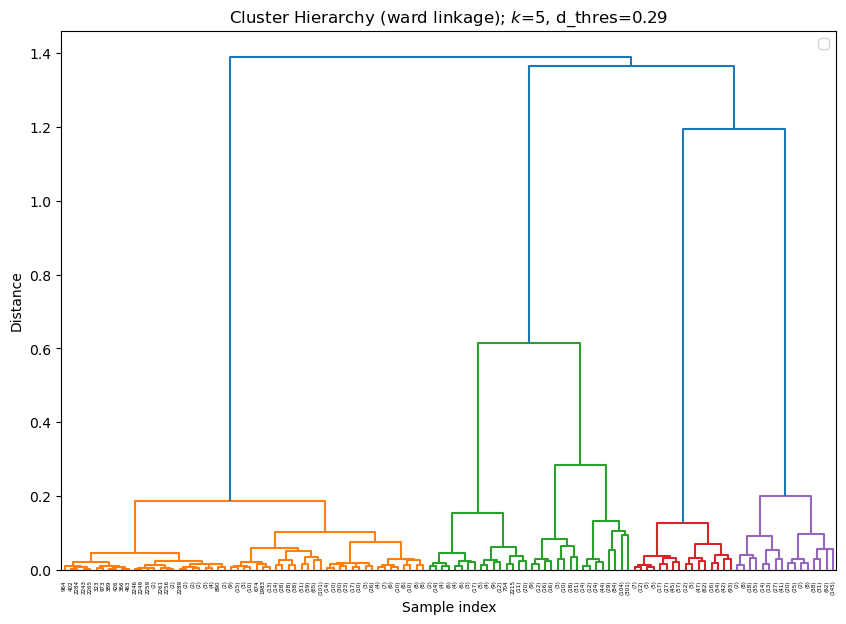
\includegraphics[scale=0.5]{img/snp_clustering_report_47_1.png}
    \end{center}
    \caption{Truncated dendrogram (6 levels) from hierarchically clustering the LD-pruned SNP data. The subtrees (inferred clusters) are a large distance from their parent splits, indicating decent separation.}
    \label{fig:hierpop}
\end{figure}

\noindent These results hint at some important characteristics of this data unaccounted for by these clustering methods. First and foremost, the distribution of pairwise distances between points is very different across the whole dataset compared to that within a single population. Ideally, the average intracluster distance that is distinct from and smaller than the average intercluster distance. This is the case across the whole dataset; but it is not the case within populations, as shown in figure $\ref{fig:pairwisedist}$.

\begin{figure}
    \begin{center}
        \begin{subfigure}[b]{0.45\textwidth}
            \centering
            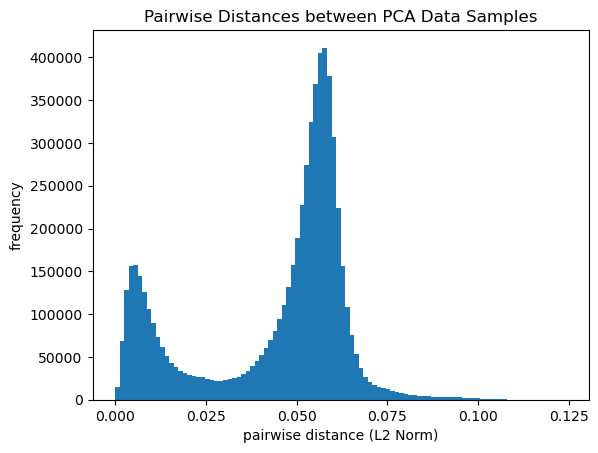
\includegraphics[width=\textwidth]{img/snp_clustering_report_24_1.png}
            \caption{pairwise distance distribution (whole dataset)}
            \label{subfig:pairwisedistwhole}
        \end{subfigure}
        \begin{subfigure}[b]{0.45\textwidth}
            \centering
            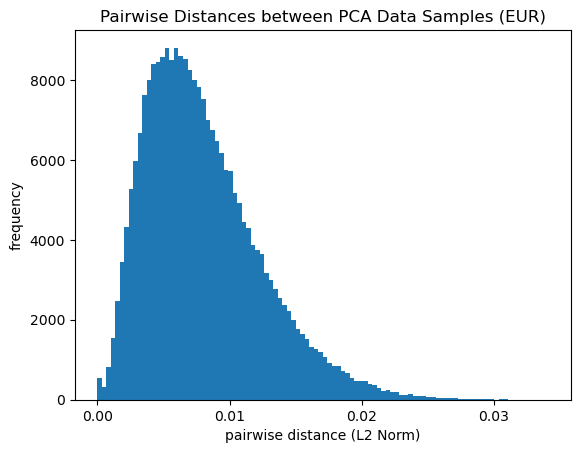
\includegraphics[width=\textwidth]{img/snp_clustering_report_26_1.png}
            \caption{pairwise distance distribution (\code{EUR})}
            \label{subfig:pairwisedisteur}
        \end{subfigure}
    \end{center}
    \caption{Distributions of pairwise distances across $\ref{subfig:pairwisedistwhole}$) the whole dataset and $\ref{subfig:pairwisedisteur}$) within the \code{EUR} population. The bimodal distribution of distances across the whole dataset makes the populations more separable than subpopulations within a single population, which have unimodally distributed pairwise distances.}
\end{figure}
\label{fig:pairwisedist}

\noindent Here we see that the distribution of pairwise distance between the data points in the entire dataset is bimodal; there is one peak (left) corresponding to intracluster distance, and another corresponding to intercluster distance. Within the \code{EUR} population the distribution of pairwise distance is unimodal, indicating indiscernible separation between subpopulations. This discrepancy is likely the reason both approaches failed to discern subpopulation structure, and further research on remedial preprocessing or clustering methods is needed.

\subsection{Limitations \& Future Research}\label{subsec:future}
\noindent This research had limitations which call for future research. Firstly, we used data from only chromosome 19. Data from more chromosomes could make subpopulation-level data more separable by adding more subpopulation-specific SNPs. Secondly, we used biologically/genetically uninformed euclidean distance on the PCA-transformed data. One could instead employ multi-dimensional scaling using custom, genetically informed pairwise distances. Thirdly, we used hierarchical clustering with a single distance threshold; the observed pairwise distances could warrant combining clusterings with multiple distance thresholds somehow, instead of taking a one-size-fits-all approach. Finally, one may want to use cluster quality score better suited for additional subcluster structure than silhouette score.

\noindent We also did not performance benchmark these methods for two reasons. First, hierarchical clustering methods have linkage-dependent asymptotic time complexities at least as slow as $k$-means. Secondly, we tuned different hyperparameters of $k$-means and hierarchical approaches. For these reasons, comparing these methods in this way would be useless at best and irresponsible at worst. We stuck with fairer comparison points like clustering quality and population structure captured.

\newpage
\bibliographystyle{plain}
\bibliography{references}
\end{document}